\documentclass[12pt,letterpaper,titlepage]{article}
\usepackage{solarized-light}
\usepackage{fontspec}
\defaultfontfeatures{Mapping=tex-text}
\usepackage{xunicode}
\usepackage{xltxtra}
\usepackage{amsmath}
\usepackage{pdfpages}
\usepackage{amsfonts}
\usepackage{amssymb}
\setcounter{secnumdepth}{0}
\usepackage{nameref}
\usepackage{enumitem}
\usepackage{environ}
\usepackage{pgfplots}
\usepackage{karnaugh-map}

\setmainfont{Times New Roman}
\showboxdepth=\maxdimen
\showboxbreadth=\maxdimen


\usepackage{paracol}
\usepackage{wrapfig}
\globalcounter{table}
\globalcounter{figure}
\usepackage{graphicx}
\usepackage[left=1in,right=1in,top=1in,bottom=1in]{geometry}
\graphicspath{{img/}}

\author{Jacob Abel}
\title{	Homework 5
	\\\large ECE3544 CRN:82989
}

\setlength{\parskip}{0.25em}

\begin{document}
\maketitle
\begin{raggedright}
\paragraph{Note: } Did not complete in time due to failure to scheduling failure.
 
\paragraph{Problem 1: }
\begin{center}
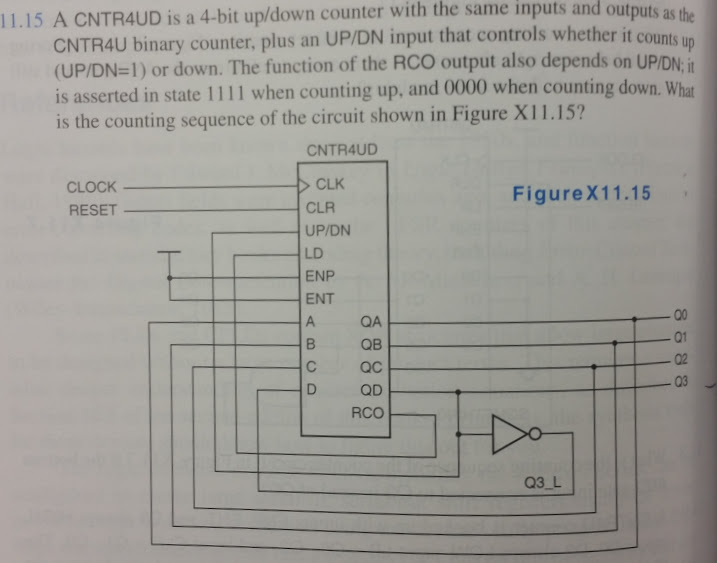
\includegraphics[width=\textwidth]{p1}
\end{center}

\paragraph{Problem 2: }
Design a modulo-16 counter, using one \texttt{CNTR4UD} (see problem 1) and at most one discrete logic gate, with the following counting sequence: 7, 6, 5, 4, 3, 2, 1, 0, 8, 9, 10, 11, 12, 13, 14, 15, 7, \ldots
\begin{center}
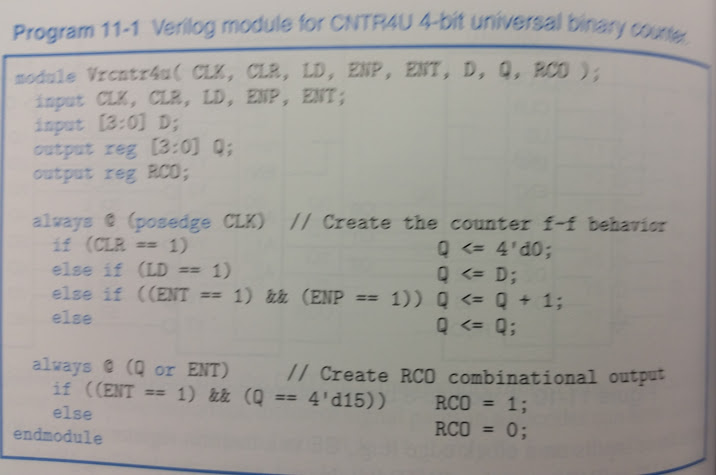
\includegraphics[width=\textwidth]{p2}
\end{center}

Create a Verilog model based upon the code in the program above 	and show the correct operation of your design.

\paragraph{Problem 3: }
\clearpage
\paragraph{Problem 4: }
Given what you know now about set-up and hold times, re-examine the circuit from project 2 and estimate the minimum clock period if the set-up time for the 74821 register is 4ns and the hold time is 2ns. You can assume the typical delays for the 7485 and the default delay for the eleven-bit counter. Below are the delays for the 7485 in nanoseconds.
 
\begin{lstlisting}
specify
  (a_in, b_in => oa_lt_b) = (16);
  (a_in, b_in => oa_gt_b) = (16);
  (a_in, b_in => oa_eq_b) = (14);
  (ia_lt_b, ia_eq_b, ia_gt_b => oa_lt_b) = (11);
  (ia_lt_b, ia_eq_b, ia_gt_b => oa_gt_b) = (11);
  (ia_gt_b => oa_eq_b) = (9);
endspecify
\end{lstlisting}

$t_{setup} = 4ns + 16ns = 20ns$

$t_{margin} = 9ns - 2ns = 7ns$

$T = 20ns + 7ns = 27ns$

$f = \frac{1}{27ns} = 37.04MHz$

\paragraph{Problem 5: }
Calculate the MTBF of the synchroniser shown in the figure below, assuming a clock frequency of 30MHz and an asynchronous transition rate of 2 MHz. Assume that the set-up time $t_{setup}$ and the propagation delay $t_{pd}$ from clock to Q or QN in a 74ALS74 are both 10ns.

\begin{center}
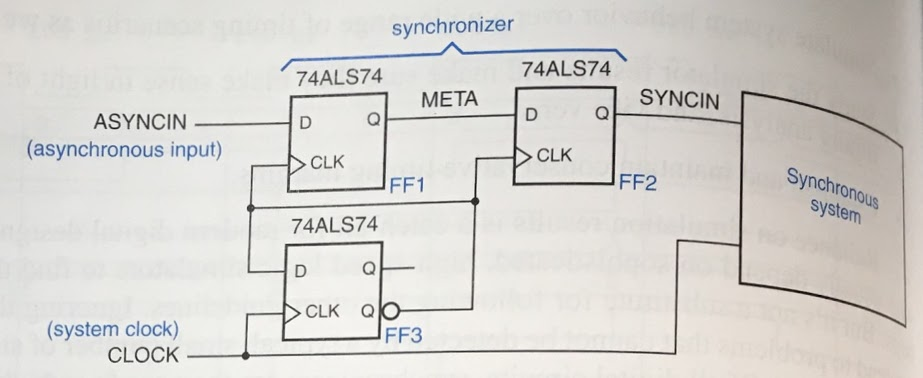
\includegraphics[width=\textwidth]{p5}
\end{center}

$t_r = \frac{1}{30MHz} - 10ns = 23.33ns$

$MTBF = e^{\frac{23.33ns}{}}$

\paragraph{Problem 6: }
Create a Verilog model of the circuit from problem 5 and verify that its operation is the same as described by your answer to problem 5. The reset signal is not shown on the schematic; you'll need to reset the flip-flops at the beginning of your simulation. You can use the D flip-flop modules from the previous homework.

\end{raggedright}
\end{document}
